\documentclass[11pt]{article}  

%%%%%%%% PREÁMBULO %%%%%%%%%%%%
\title{Portada reporte practicas}

\usepackage{tikz}
\usetikzlibrary{positioning, arrows.meta}
\usetikzlibrary{shapes.geometric, arrows}
\usetikzlibrary{positioning, arrows.meta}
\usetikzlibrary{positioning, arrows.meta}
\usepackage[spanish]{babel} 
\usepackage[utf8]{inputenc}    
\usepackage{amsmath} 
\usepackage{xcolor}

%\usepackage{amssymb} 
\usepackage{graphicx} 
\usepackage{color} 
\usepackage{subfigure} 
\usepackage{float} 
\usepackage{capt-of} 
\usepackage{sidecap} 
	\sidecaptionvpos{figure}{c} 
\usepackage{caption} 
\usepackage{commath}  

\usepackage{cancel} 
 
\usepackage{anysize} 					
\marginsize{2cm}{2cm}{2cm}{2cm} 

\usepackage{appendix}
\renewcommand{\appendixname}{Apéndices}
\renewcommand{\appendixtocname}{Apéndices}
\renewcommand{\appendixpagename}{Apéndices} 

\usepackage[colorlinks=true,plainpages=true,citecolor=blue,linkcolor=blue]{hyperref}

\usepackage{fancyhdr} 
\pagestyle{fancy}
\fancyhf{}
\fancyhead[L]{\footnotesize UPIITA} 
\fancyhead[R]{\footnotesize IPN}   
\fancyfoot[R]{\footnotesize Programacion Avanzada}  
\fancyfoot[C]{\thepage} 
\fancyfoot[L]{\footnotesize Ing. Mecatrónica}  
\renewcommand{\footrulewidth}{0.4pt}


\usepackage{listings} 
\definecolor{dkgreen}{rgb}{0,0.6,0} 
\definecolor{gray}{rgb}{0.5,0.5,0.5}

\tikzstyle{startstop} = [rectangle, rounded corners, minimum width=3cm, minimum height=1cm,text centered, draw=black, fill=red!30]
\tikzstyle{process} = [rectangle, minimum width=3cm, minimum height=1cm, text centered, draw=black, fill=orange!30]
\tikzstyle{io} = [trapezium, trapezium left angle=70, trapezium right angle=110, minimum width=3cm, minimum height=1cm, text centered, draw=black, fill=blue!30]
\tikzstyle{decision} = [diamond, minimum width=3cm, minimum height=1cm, text centered, draw=black, fill=green!30]
\tikzstyle{arrow} = [thick,->,>=stealth] 

% configuración para el lenguaje que queramos utilizar
\lstnewenvironment{python}[1][]
{
    \lstset{
        language=Python,
        basicstyle=\small\ttfamily,
        keywordstyle=\color{blue}\bfseries,
        commentstyle=\color{green!60!black},
        stringstyle=\color{red},
        showstringspaces=false,
        frame=single,
        numbers=left,
        numberstyle=\tiny,
        numbersep=5pt,
        #1
    }
}
{}
\title{Plantilla portada}

%%%%%%%% TERMINA PREÁMBULO %%%%%%%%%%%%

\begin{document}

%%%%%%%%%%%%%%%%%%%%%%%%%%%%%%%%%% PORTADA %%%%%%%%%%%%%%%%%%%%%%%%%%%%%%%%%%%%%%%%%%%%
																					%%%
\begin{center}																		%%%
\newcommand{\HRule}{\rule{\linewidth}{0.5mm}}									%%%\left
 																					%%%
 																					
\begin{minipage}{0.48\textwidth} \begin{flushleft}

\includegraphics[scale = 0.63]{logo_upiita.png}
\end{flushleft}\end{minipage}
\begin{minipage}{0.48\textwidth} \begin{flushright}

\includegraphics[scale = 0.35]{IPN.jpg}
\end{flushright}\end{minipage}

													 								%%%
\vspace*{-1.5cm}								%%%
																					%%%	
\textsc{\huge Instituto Polit\'ecnico\\ \vspace{5px} Nacional}\\[1.5cm]	

\textsc{\LARGE Unidad Profesional Interdisciplinaria en Ingenier\'ia y				%%%
Tecnolog\'ias Avanzadas}\\[1.5cm]													%%%

\begin{minipage}{0.9\textwidth} 
\begin{center}																					%%%
\textsc{\LARGE Programación Avanzada 2MV7}
\end{center}
\end{minipage}\\[0.5cm]
%%%
    																				%%%
 			\vspace*{1cm}																		%%%
																					%%%
\HRule \\[0.4cm]																	%%%
{ \huge \bfseries Practica 5}\\[0.4cm]	%%%
 																					%%%
\HRule \\[1.5cm]																	%%%
 																				%%%
																					%%%
\begin{minipage}{0.46\textwidth}													%%%
\begin{flushleft} \large															%%%
\emph{Autor:}\\	
Barrios Mendez Jose Alberto\\
Boleta: 2022640111


%%%
			%\vspace*{2cm}	
            													%%%
										 						%%%
\end{flushleft}																		%%%
\end{minipage}		
																%%%
\begin{minipage}{0.52\textwidth}		
\vspace{-0.6cm}											%%%
\begin{flushright} \large															%%%
\emph{Profesor:} \\																	%%%
Cruz Mora Jose Luis\\
													%%%
\end{flushright}																	%%%
\end{minipage}	
\vspace*{1cm}
%\begin{flushleft}
 	
%\end{flushleft}
%%%
 		\flushleft{\textbf{\Large Ing. Mecatrónica}	}\\																		%%%
\vspace{2cm} 																				
\begin{center}																					
{\large \today}																	%%%
 			\end{center}												  						
\end{center}							 											
																					
\newpage																		
%%%%%%%%%%%%%%%%%%%% TERMINA PORTADA %%%%%%%%%%%%%%%%%%%%%%%%%%%%%%%%

\tableofcontents 

\newpage

\section{Objetivo.}
Crear aplicaciones con interfaces gráficas de usuario (GUI) utilizando los controles avanzados.

\section{Introduccion.} 
Para esta practica numero 5, nos proponen un reto, el cual consiste en reutilizar la practica de la tienda de mascotas para crear una interfaz de usuario en la cual se lleve a cabo la implementacion para la venta de las mascotas requeridas en la practica anteriormente solicitada. Sin embargo el reto aqui es desarrollar la practica en una interfaz de usuario (GUI) con la ayuda de PyQt6, podremos hacer el diseño de la interfaz de una forma mas amigable, recordando que PyQt6 tiene como objetivo el diseño de interfaces. Una vez que hayamos elegido el diseño de nuestra interfaz es neccesario llevar a cabo el back-end, para que nuestra interfaz de usuario funcione de una forma  optima
\section{Desarrollo.}

\subsection{Creacion de la interfaz}

Con ayuda del designer de PyQt6, creamos la siguiente interfaz grafica en el entorno
\begin{figure}[H]
		\begin{center}
 			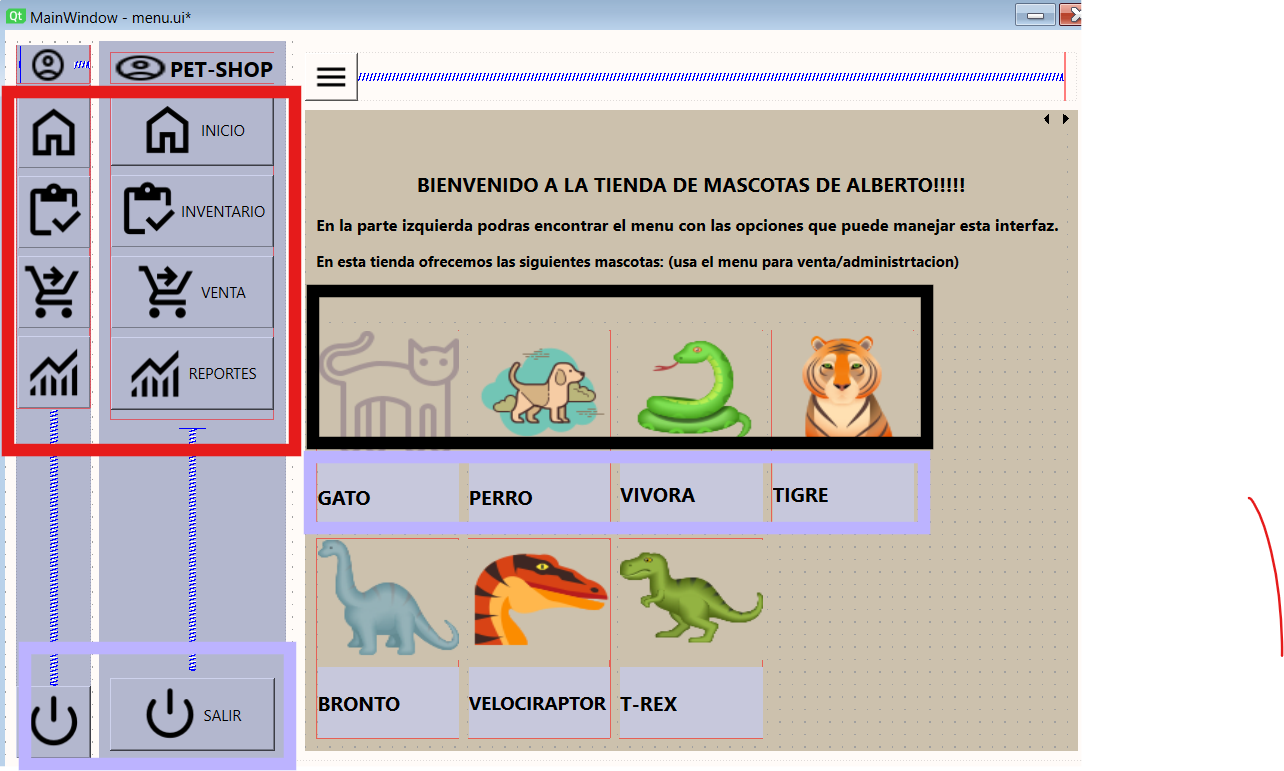
\includegraphics[width = .8\textwidth]{01.png}
 			\captionof{figure}{\label{fig:IPN}Interfaz diseñada en PyQt6-Designer} 
 			
		\end{center} 
\end{figure}
En la imagen podemos observar distintos elementos, empezando por los elementos encerrados en el recuadro de color rojo, los cuales son elementos de tipo Pushbuttom, tienen como funcionalidad o proposito el cambiar entre distintas ventanas de la interfaz grafica, esto lo trataremos mas a detalle mas adelante. Continuando con los elementos dentro de esta primera interfaz tambien notamos elementos de tipo QLael, los cuales me sirven como contenerdores o como elementos para poder representar o ubicar una imagen dentro de estos, ademas de poder colocar texto en estos elementos de la interfaz.
Es importante mencionar que dentro  de tod o el menu de color parecido al morado, este va a ser un menu desplegable, el cual se activara al presionar el simbolo de menu, o algunas de los elementos del menu, para poder llevar a cabo esto, es necesario hacer lo siguiente: 

\begin{figure}[H]
		\begin{center}
 			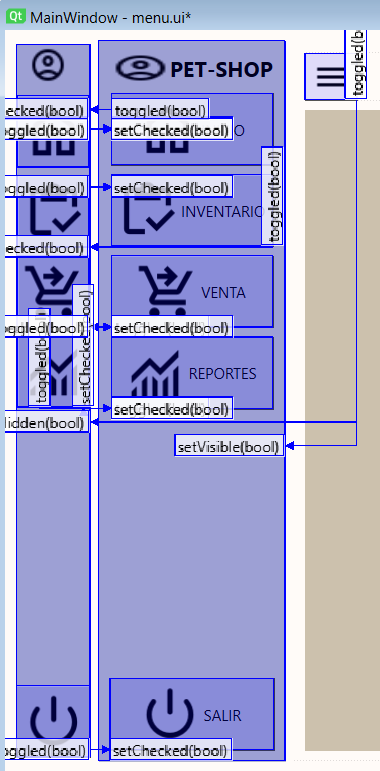
\includegraphics[width = .4\textwidth]{06.png}
 			\captionof{figure}{\label{fig:IPN}Conexion entre elementos dentro de la interfaz grafica} 
 			
		\end{center} 
\end{figure}

Aqui tenemos algunas funciones a destacar

setCheckable(bool): Este método se utiliza para especificar si un elemento del menú es seleccionable o no. Si se establece como True, el elemento será seleccionable y tendrá un estado de verificación, lo que significa que el usuario puede marcar o desmarcar el elemento. Si se establece como False, el elemento no será seleccionable.

setChecked(bool): Este método se utiliza para establecer el estado de verificación de un elemento del menú. Si el elemento es checkable (seleccionable), setChecked(True) lo marcará, y setChecked(False) lo desmarcará.

setVisible(bool): Este método se utiliza para controlar la visibilidad de un elemento del menú. Si se establece como True, el elemento será visible en el menú desplegable. Si se establece como False, el elemento estará oculto y no será visible para el usuario en el menú.

En el caso de las diferentes ventanas dentro de la interfaz es suficiente con usar un stack widget. Un "stacked widget" es útil cuando se quiere mostrar diferentes vistas o pantallas en una misma área de la interfaz de usuario, pero solo quieres que una de ellas sea visible a la vez. Por ejemplo, podría tener un formulario de registro con varias páginas. Para nuestra interfaz nos sevira para poder tener las paginas de cada uno de los botones del menu mostrado anteriormente:



\begin{figure}[H]
		\begin{center}
 			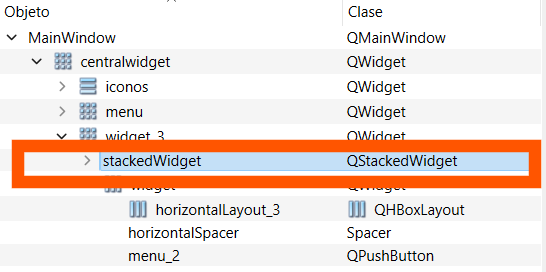
\includegraphics[width = .2\textwidth]{05.png}
 			\captionof{figure}{\label{fig:IPN}elemento para poder almacenar varias paginas} 
 			
		\end{center} 
\end{figure}

Aunque la parte del diseño juega un papel crucial dentro del desarollo de la practica, es importante conocer el como estan implementados los elementos dentro del codigo, o mejor dicho, saber el como funcionara interiormente. Aunque esta primera pagina no requiere mucha ciencia para describir el funcionamiento, ya que todos los elementos son estaticos y no van a cambiar, es importante conocer como funcionan la parte del menu, veamos como esta implementado
\begin{figure}[H]
		\begin{center}
 			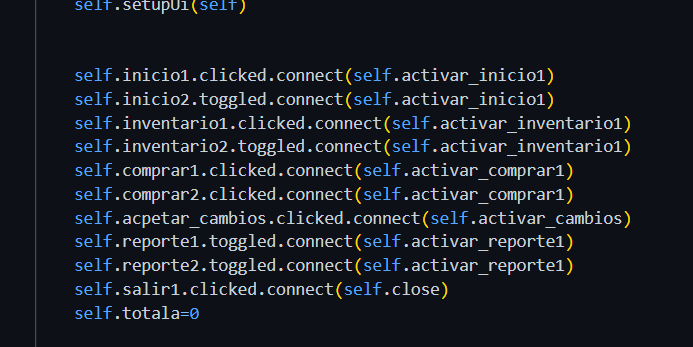
\includegraphics[width = .5\textwidth]{07.png}
 			\captionof{figure}{\label{fig:IPN}Conexion de la señales "clicked" con una funcion}
 			 
 			
		\end{center} 
\end{figure}

Para empezar conectamos cada señal que puedan hacer los botones, es decir, al momento que se detecte un click sobre estos botones, vamos a mandar a llamar una a una funcion que se encargara de realizar la accion, para esta primera parte solo nos activara alguna pagina del stack widget :
\begin{figure}[H]
		\begin{center}
 			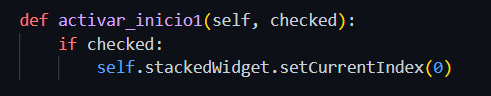
\includegraphics[width = .5\textwidth]{08.png}
 			\captionof{figure}{\label{fig:IPN}Funcion para activar una pagina del stacked widget} 
 			
		\end{center} 
\end{figure}

Aqui podemos ver que al llevar acabo el evento se manda a llamar la respectiva funcion  de cada boton, aqui entra en juego el concepto de indice del stacked widget, el cual empieza con cero, entonces la pagina numero 1, tendra el indice cero

Ahora continuemos con nuestra segunda ventana de la interfaz grafica:
\begin{figure}[H]
		\begin{center}
 			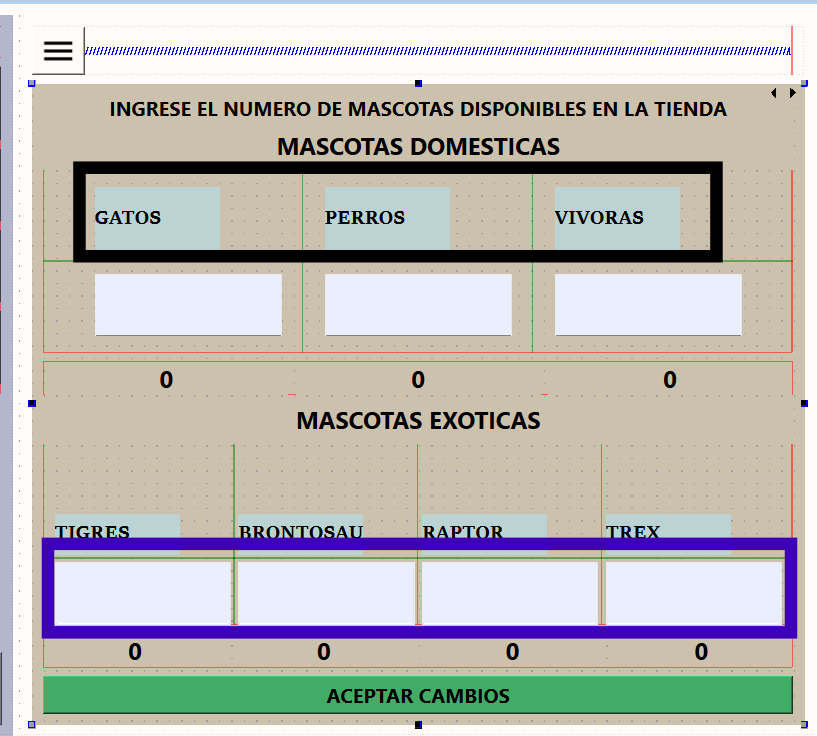
\includegraphics[width = .7\textwidth]{02.png}
 			\captionof{figure}{\label{fig:IPN}Interfaz para poder configurar el inventario} 
 			
		\end{center} 
\end{figure}


En este caso podemos observar que los elementos encerrados en el recuadro de color negro son elementos de tipo QLabel, se mantendran estaticos y no se actualizaran, tambien hay algunos elementos en blanco, los cuales son de tipo EditText, en estos recuadros el usuario ingresara el numero de mascatos de cada tipo que tiene, ademas los valores que en un inicio estan marcados con cero, se actualizaran al numero ingresado cuando se presione  el boton de color verde  "ACEPTAR CAMBIOS"\\
Veamos que hay en la implementacion del codigo para esta ventanda, recordando que la señal clicked ya esta conectada a la funcion siguiente: 
\begin{figure}[H]
		\begin{center}
 			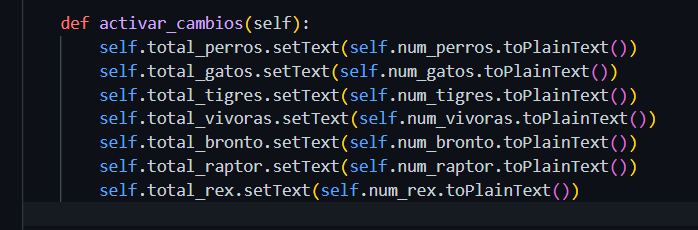
\includegraphics[width = .7\textwidth]{09.png}
 			\captionof{figure}{\label{fig:IPN}Funcion de aceptar cambios } 
 			
		\end{center} 
\end{figure}

Para esta funcion es algo sencillo, solo actualizar valores dentro de los QLabels
 self.totalperros.setText(self.numperros.toPlainText()): Esto actualiza el texto del widget totalperros con el contenido del widget de entrada de texto numperros. \\
De forma similar aplica para el resto de QLabels

Ademas de este metodo, se agrego otro metodo el cual tiene como funcion ser un filtro, donde analizara la entrada del teclado y en caso de ingresar una tecla diferente a un numero, mandara un mensaje de error, la funcion de filtro es la siguiente: 
\begin{figure}[H]
		\begin{center}
 			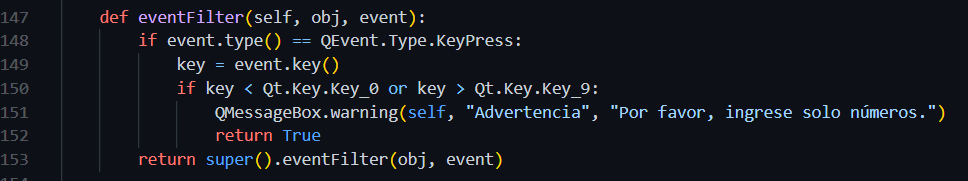
\includegraphics[width = .7\textwidth]{10.png}
 			\captionof{figure}{\label{fig:IPN}Metodo para filtrar la entrada de teclado} 
 			
		\end{center} 
\end{figure}

Una vez que hemos hecho las primeras 2 paginas, pasaremos a la tercera la cual se muestra a continuacion: 

\begin{figure}[H]
		\begin{center}
 			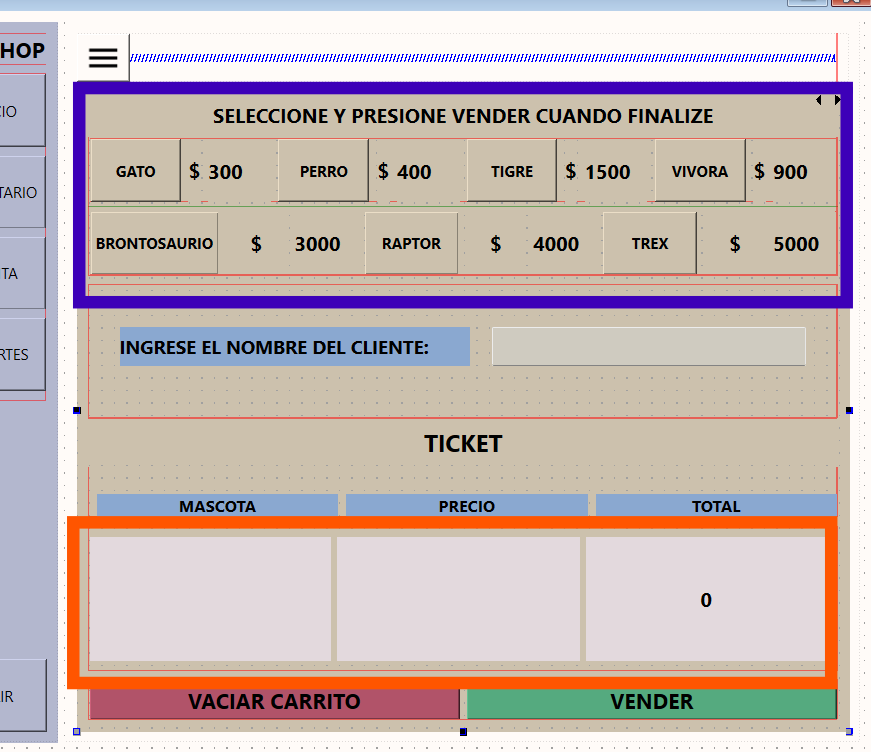
\includegraphics[width = .7\textwidth]{03.png}
 			\captionof{figure}{\label{fig:IPN}Ventana para llevar acabo las ventas de la tienda} 
 			
		\end{center} 
\end{figure}

En esta ventana observemos que tenemos las mascotas disponibles en la parte superior( recuadro de color azul), en la parte inferior (recuadro rojo) tenemos 3 elementos que se iran actualizando conforme se agreguen los elementos al carrito, los cuales simularan una especie de ticked, que posteriormente se imprimira.\\
En la parte de la implementacion del codigo tendremos lo siguiente: 

\begin{figure}[H]
		\begin{center}
 			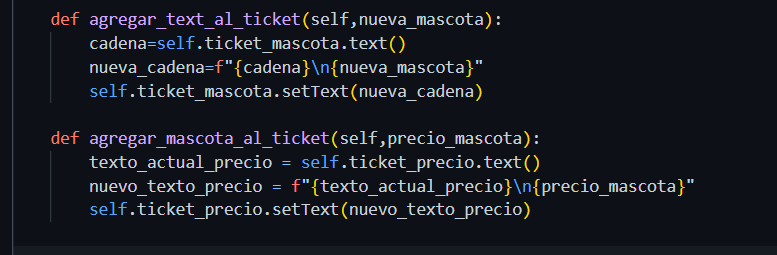
\includegraphics[width = .7\textwidth]{11.png}
 			\captionof{figure}{\label{fig:IPN}Actualizar los elementos en el carrito} 
 			
		\end{center} 
\end{figure}

agregartextalticket(self, nuevamascota): Esta función agrega un nuevo texto al widget ticketmascota. Toma el texto actual del widget, concatena el texto de la nueva mascota al final, y luego actualiza el texto del widget ticketmascota con la nueva cadena.

cadena = self.ticketmascota.text(): Obtiene el texto actual del widget ticketmascota.

nuevacadena = f"{cadena}{nuevamascota}": Crea una nueva cadena que consiste en el texto original del widget ticketmascota seguido de un salto de línea  y el texto de la nueva mascota.

self.ticketmascota.setText(nuevacadena): Establece el texto del widget ticketmascota como la nueva cadena creada.

agregarmascotaalticket(self, preciomascota): Esta función agrega un nuevo precio al widget ticketprecio. Similar a la función anterior, toma el texto actual del widget, concatena el precio de la nueva mascota al final, y luego actualiza el texto del widget ticketprecio con la nueva cadena.
textoactualprecio = self.ticketprecio.text(): Obtiene el texto actual del widget ticketprecio.

nuevotextoprecio = f"{textoactualprecio}{preciomascota}": Crea una nueva cadena que consiste en el texto original del widget ticketprecio seguido de un salto de línea  y el precio de la nueva mascota.

self.ticketprecio.setText(nuevotextoprecio): Establece el texto del widget ticketprecio como la nueva cadena creada.

Para el metodo que se activara cuando se presione un boton con el nombre de la mascota tendremos funciones parecidas a la siguiente con cada boton

\begin{figure}[H]
		\begin{center}
 			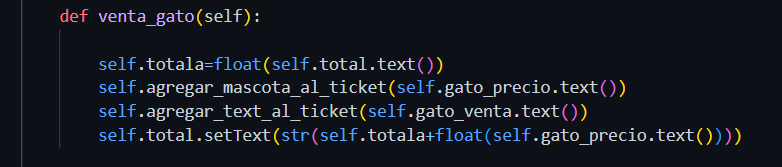
\includegraphics[width = .6\textwidth]{12.png}
 			\captionof{figure}{\label{fig:IPN}Metodo para venta de mascotas} 
 			
		\end{center} 
\end{figure}

self.totala = float(self.total.text()): Obtiene el texto actual del widget total, lo convierte a un valor flotante y lo asigna a la variable self.totala.

self.agregarmascotaalticket(self.gatoprecio.text()): Llama a la función agregarmascotaalticket (que explicamos anteriormente) para agregar el precio del gato al ticket. Toma el texto actual del widget gatoprecio  y lo pasa como argumento a la función.

self.agregartextalticket(self.gatoventa.text()): Llama a la función agregartextalticket (también explicada anteriormente) para agregar el texto relacionado con la venta del gato al ticket. Toma el texto actual del widget gatoventa y lo pasa como argumento a la función.

self.total.setText(str(self.totala + float(self.gatoprecio.text()))): Actualiza el texto del widget total sumando el precio del gato al valor previamente almacenado en self.totala. Primero convierte el texto actual del widget gatoprecio a un valor flotante, luego suma este valor al valor previamente almacenado en self.totala, y finalmente convierte el resultado de vuelta a una cadena antes de establecerlo como el nuevo texto del widget total.

Una vez que hemos explicado el funcionamiento de las ventanasd e la interfaz grafica, procederemos a vizualizar los resultados

\section{Resultados.}

En esta parte de resultados vamos a ejecutar nuestro archivo .py, con las implementaciones en el codigo, anteriormente mencionadas

\begin{figure}[H]
		\begin{center}
 			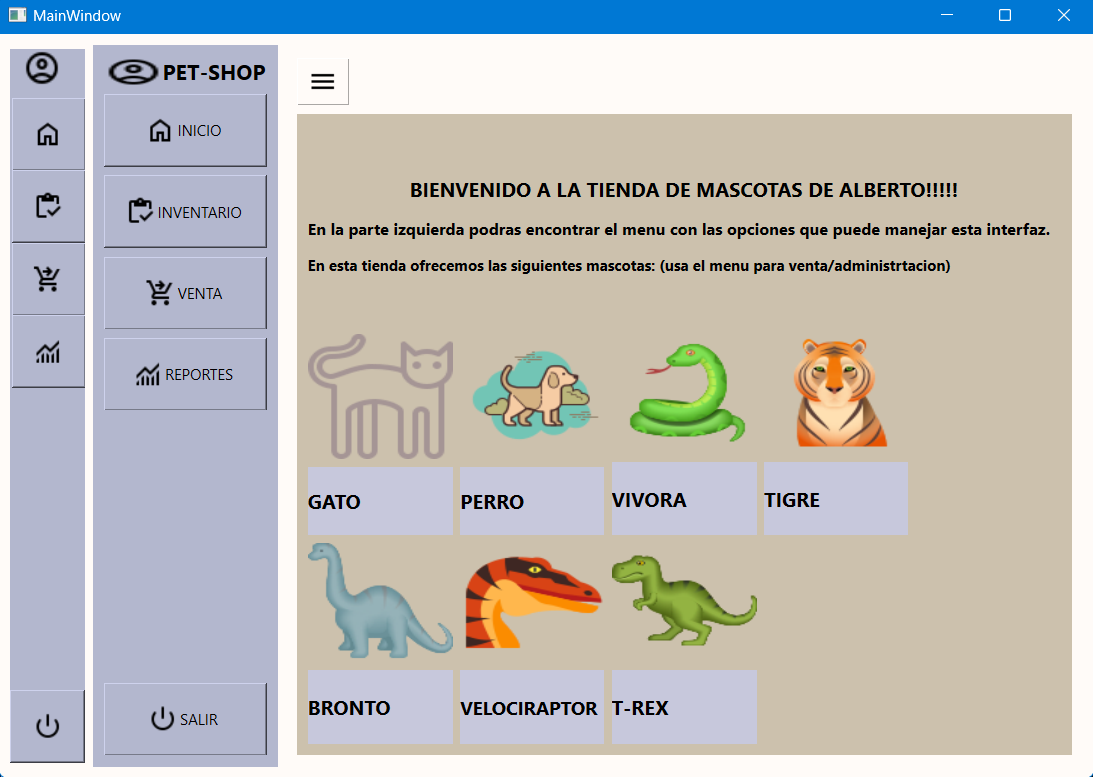
\includegraphics[width = .6\textwidth]{13.png}
 			\captionof{figure}{\label{fig:IPN}Ventana de inicio de la interfaz} 
 			
		\end{center} 
\end{figure}

\begin{figure}[H]
		\begin{center}
 			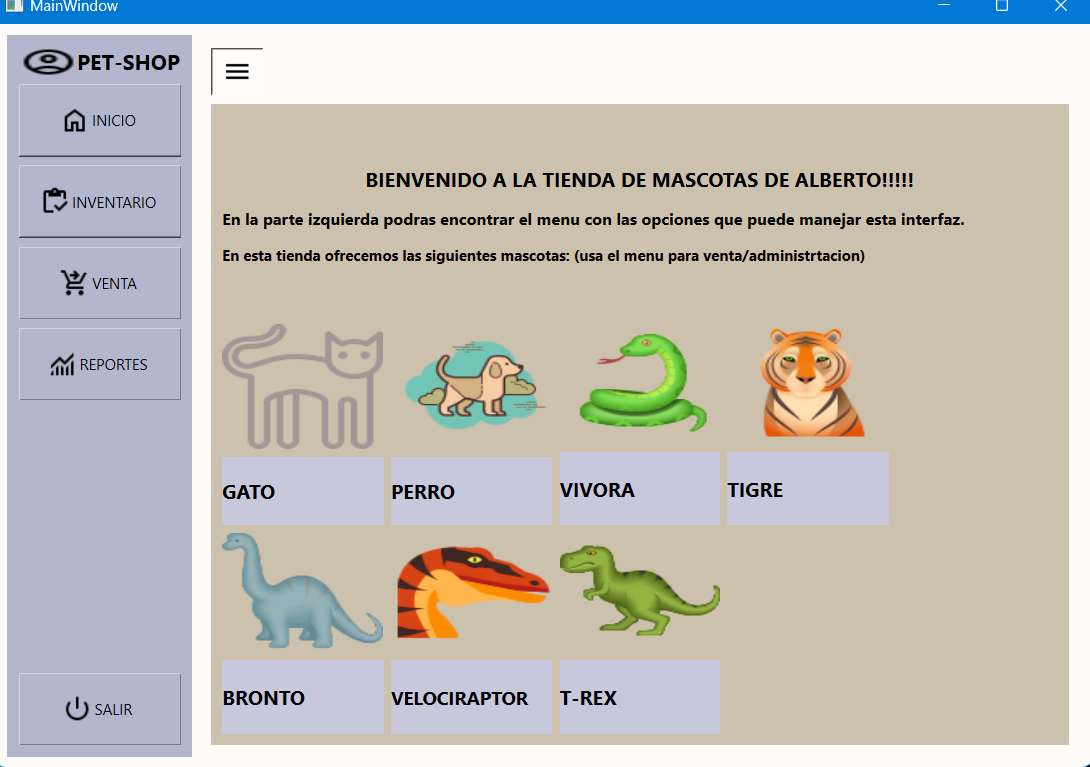
\includegraphics[width = .6\textwidth]{14.png}
 			\captionof{figure}{\label{fig:IPN}click en el simbolo de menu} 
 			
		\end{center} 
\end{figure}

\begin{figure}[H]
		\begin{center}
 			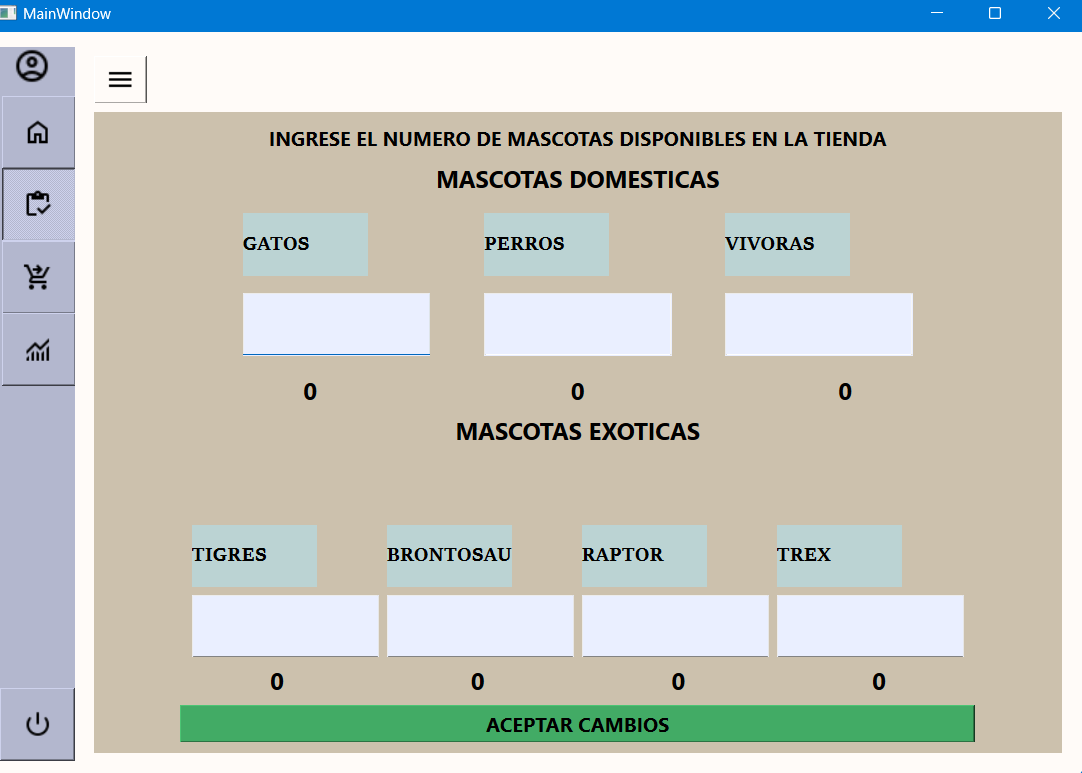
\includegraphics[width = .6\textwidth]{15.png}
 			\captionof{figure}{\label{fig:IPN}Ventana para modificar el inventario.} 
 			
		\end{center} 
\end{figure}

\begin{figure}[H]
		\begin{center}
 			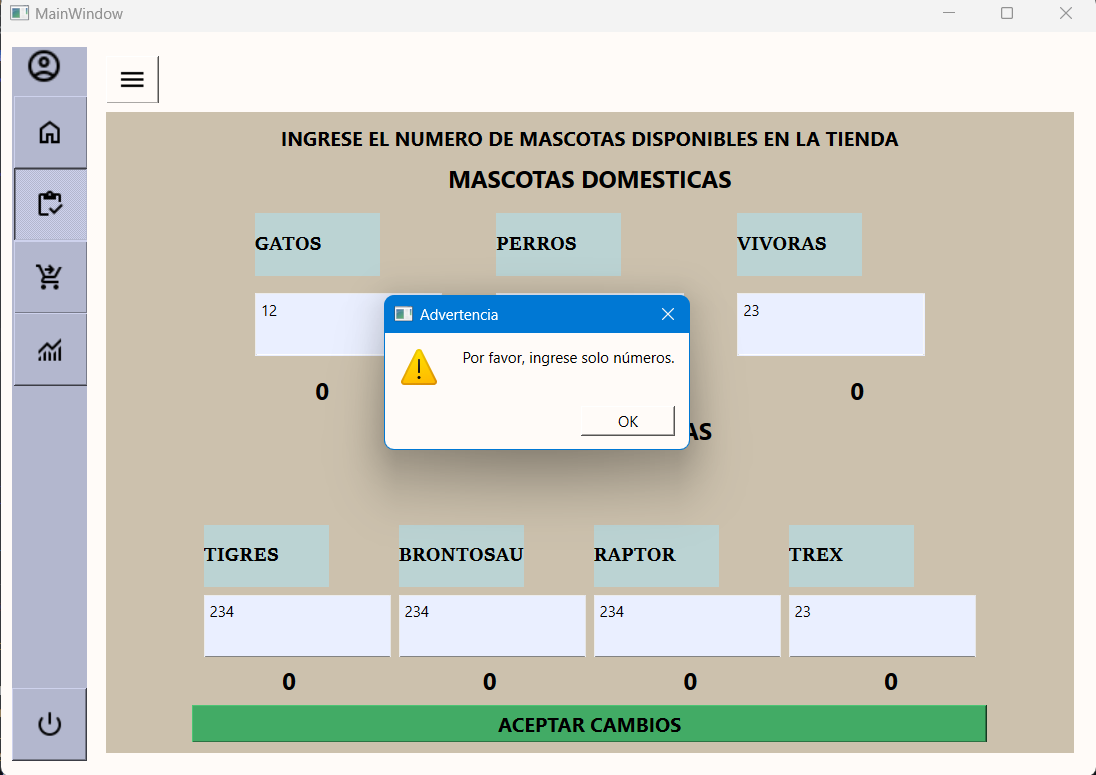
\includegraphics[width = .6\textwidth]{16.png}
 			\captionof{figure}{\label{fig:IPN}Intento de igresar dato erroneo} 
 			
		\end{center} 
\end{figure}

\begin{figure}[H]
		\begin{center}
 			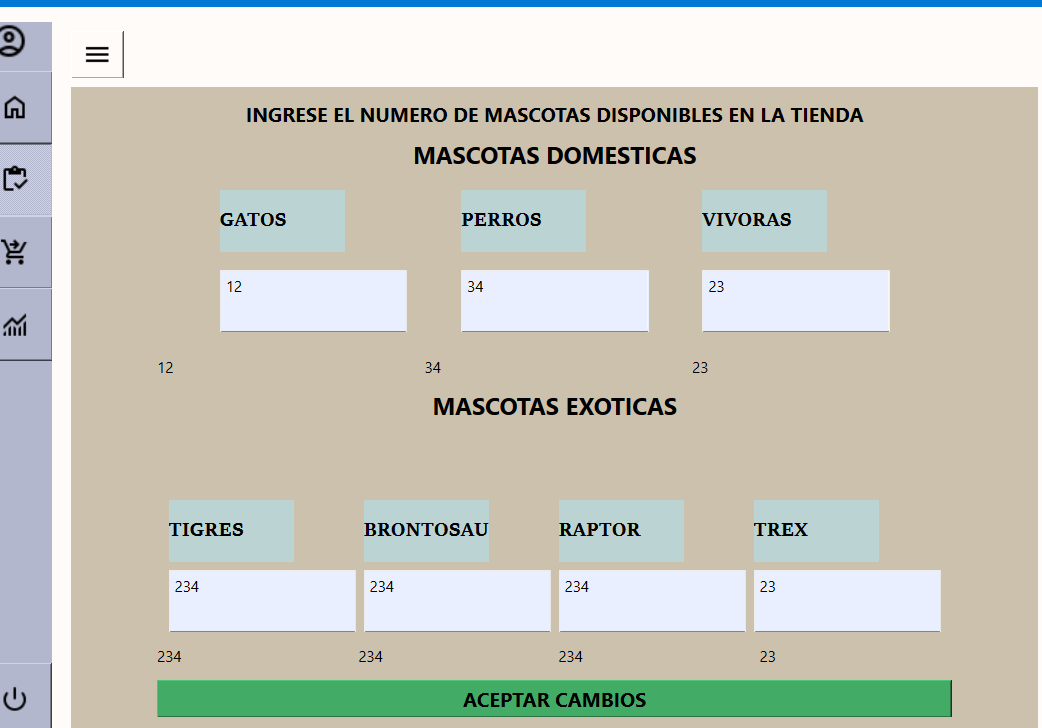
\includegraphics[width = .6\textwidth]{17.png}
 			\captionof{figure}{\label{fig:IPN}Actualizacion en el numero de animales, una vez presionado ACEPTAR CAMBIOS} 
 			
		\end{center} 
\end{figure}

\begin{figure}[H]
		\begin{center}
 			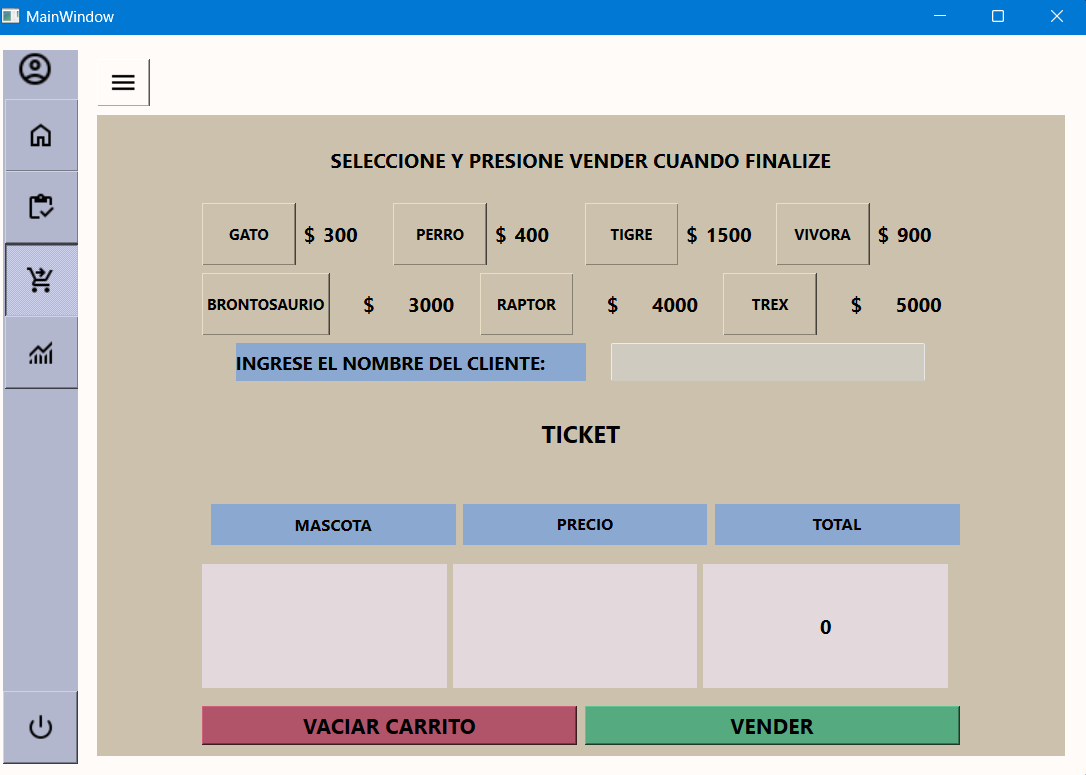
\includegraphics[width = .6\textwidth]{18.png}
 			\captionof{figure}{\label{fig:IPN}Ventana para la opcion de vender mascotas} 
 			
		\end{center} 
\end{figure}

\begin{figure}[H]
		\begin{center}
 			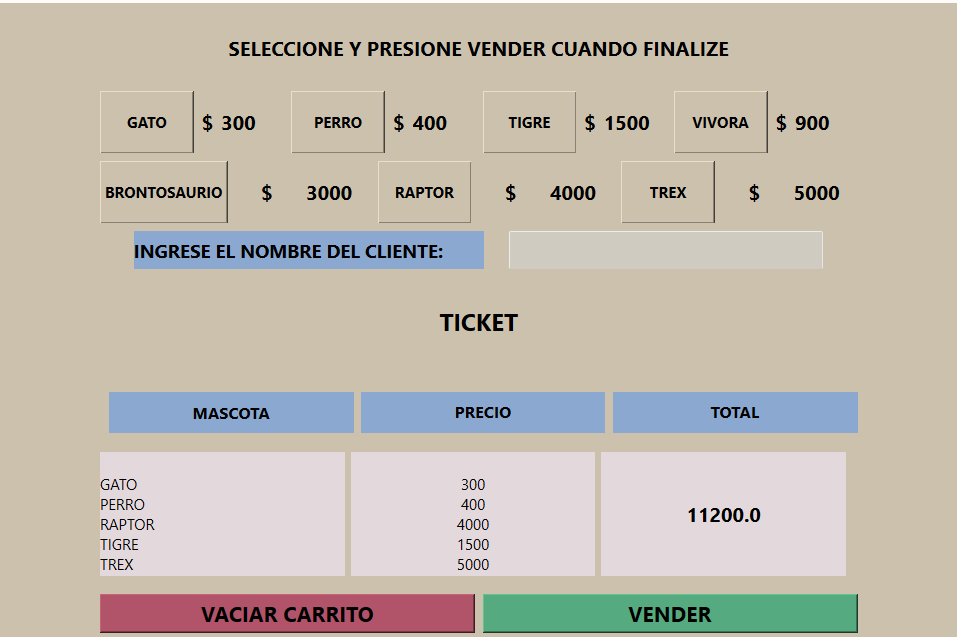
\includegraphics[width = .6\textwidth]{19.png}
 			\captionof{figure}{\label{fig:IPN}Agregar mascotas al carrito} 
 			
		\end{center} 
\end{figure}

\begin{figure}[H]
		\begin{center}
 			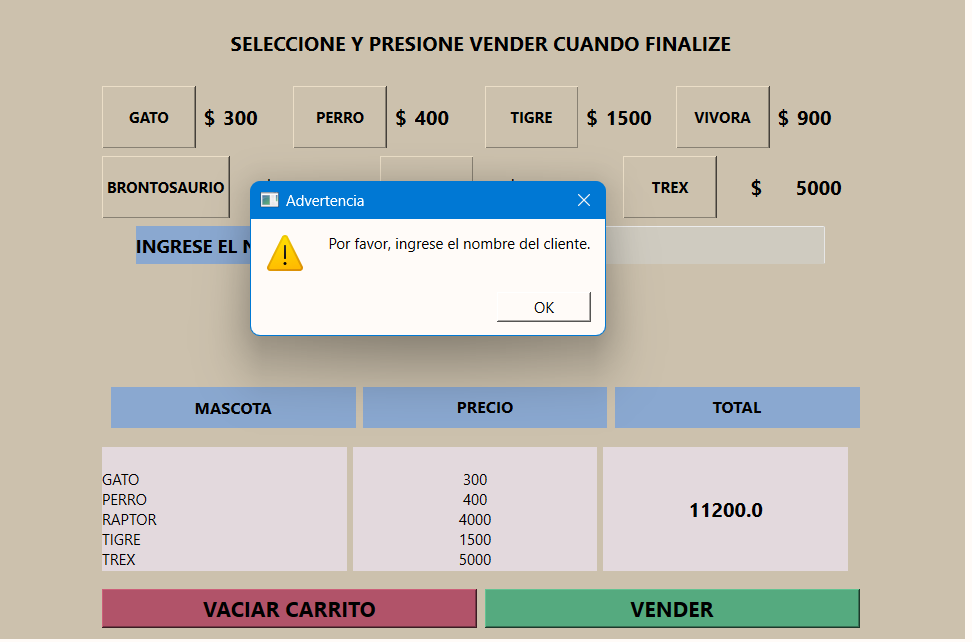
\includegraphics[width = .6\textwidth]{20.png}
 			\captionof{figure}{\label{fig:IPN}Intentar presionar el boton de vender, sin ingresar el nombre del cliente.} 
 			
		\end{center} 
\end{figure}

\begin{figure}[H]
		\begin{center}
 			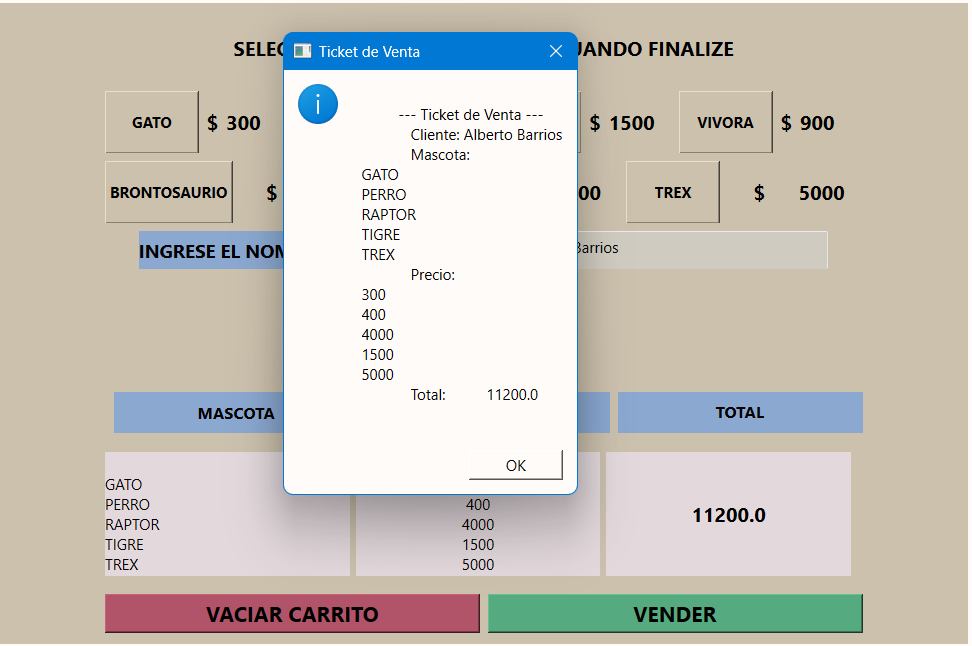
\includegraphics[width = .6\textwidth]{21.png}
 			\captionof{figure}{\label{fig:IPN}Una vez ingreado nos muestra el ticket de venta} 
 			
		\end{center} 
\end{figure}

\begin{figure}[H]
		\begin{center}
 			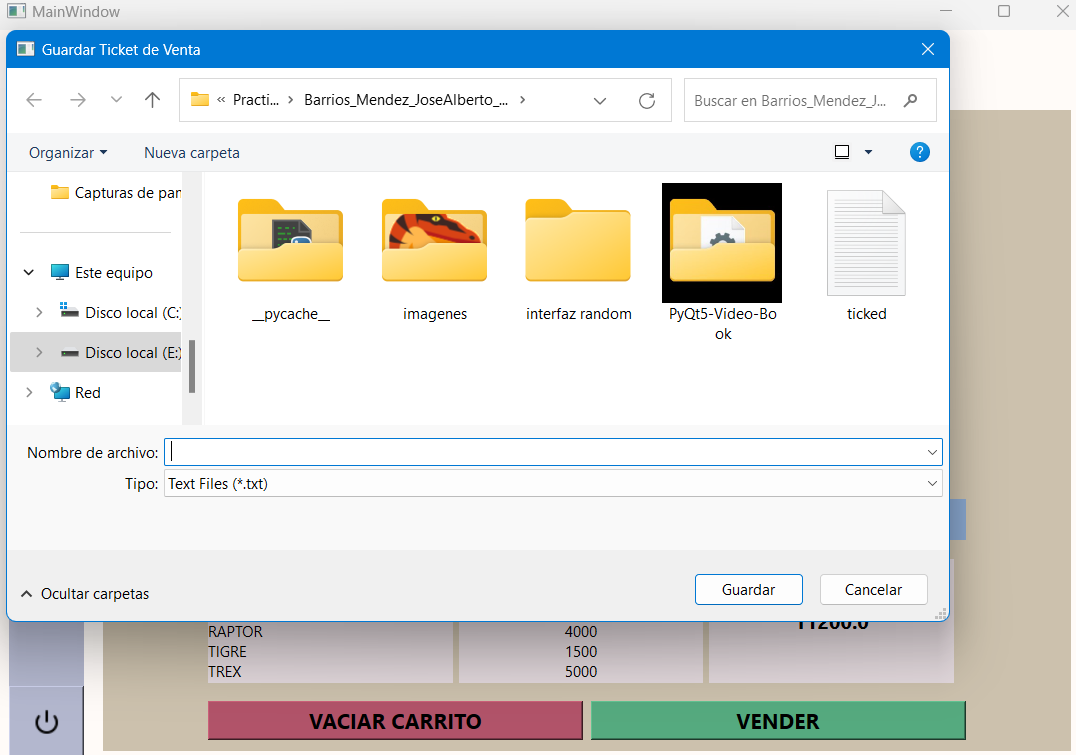
\includegraphics[width = .6\textwidth]{22.png}
 			\captionof{figure}{\label{fig:IPN}Al presionar OK, nos manda a una ventana para poder guardar el ticket como archivo .txt} 
 			
		\end{center} 
\end{figure}

\begin{figure}[H]
		\begin{center}
 			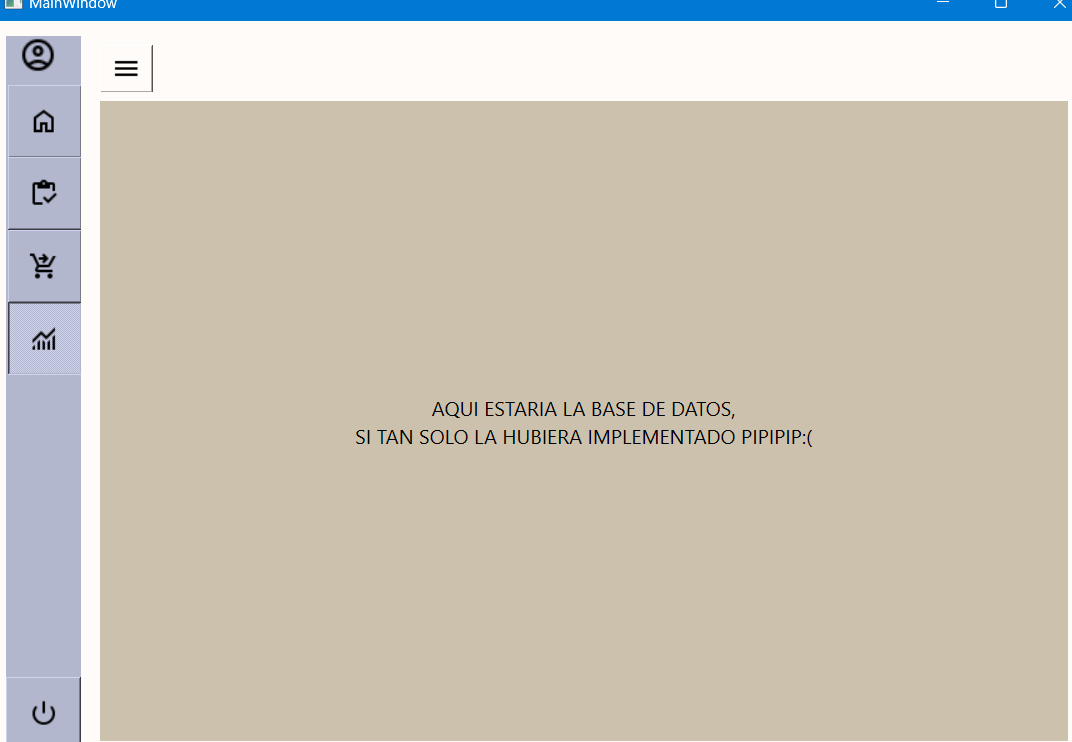
\includegraphics[width = .6\textwidth]{23.png}
 			\captionof{figure}{\label{fig:IPN}No medi bien mi tiempo profe:(} 
 			
		\end{center} 
\end{figure}

\newpage
\section{Conclusiones.}
Al realizar esta practica me e dado cuenta que la forma de realizar las interfaces graficas es un proceso sumamente complicado, en el ambito de lograr obtener un buen diseño, ya que es necesario considerar o verlo desde un punto de vista a nivel de usuario, es decir, imaginar que tu eres el usuario para poder plaenear de una mejor forma la interfaz, y de esta forma lograr obtener una buena interfaz.\\
De esta forma se llega a la clonclusion que lo mas complicado es hacer el diseño, de igual forma, conforme estas avanzando con la interfaz te das cuenta de que mas cosas se le puede agregar, o al menos en mi caso, fue sobre la marcha donde me iba dando cuenta que necesitaba algun otro elemento para poder hacer mas facil la implementacion del codigo, sin embargo por falta de administracion de tiempo, eh dejado imcompleta esta practica, pero aun asi me quedo con el conocimiento obtenido para lograr los avances en la interfaz




%%%%%%% Bibliografía %%%%%%%%    

%\appendix  
%\clearpage % o \cleardoublepage
%\addappheadtotoc 
%\appendixpage

%\section{Anexos 1.}




%\section{Anexos 2.}


 

\end{document}
